\section{Sprint 3}

\subsection{Sprint planning}
	In sprint 3 the group planned to implement the final requirements with high priority, as well as most of the requirements with medium priority. This is the second to last sprint, and it is important that in the last sprint the  only remaining requirements are medium to low requirements, so that time can also be spent fixing bugs and make the game work properly on iOS. The goal for this sprint will be to get a fully playable game, with only minor requirements missing.

	A usability test will be carried out in the last week of the sprint to discover potential bugs or errors we have yet to discover, as well as ideas for improvements that may be implemented in the next sprint.

	Concerning the report, we plan to finish the chapters up until this sprint.

\subsection{Duration and Workload}
	
	{\bf Duration:} 14.10 - 27.10 (2 weeks)\\
	{\bf Workload:} This is the list with hours spent (the whole group) on the project in this sprint.
	\begin{itemize}
		\item {\bf Planning:} 15.5 hours
		\item {\bf Development:} 44 hours
		\item {\bf Design:} 0 hours
		\item {\bf Documentation (report):} 59.5 hours
		\item {\bf Testing:} 20.5 hours 
	\end{itemize}
	{\bf Total workload: } 139.5 hours \\
	
	The group's goal was to work at least 20 hours per person every week in this sprint. 
	The group did manage the a workload with an average of 17.4 hours/week (139.5 hours/4 persons/2 weeks = 20.6 hours). The reason for the low numbers is because one of the group members did not
	participate as much as he should. The 3 other group members did work over 20 hours. 


\clearpage
\subsection{Sprint Backlog}
	\begin{table}[H]
	\begin{tabular}{| p{1cm} | p{7cm} | p{2cm} | p{2cm} |}
		\hline
		\rowcolor{gray}
		ID & Description & Estimate & Actual effort \\ \hline

		FR2.5 & The amount of power available to the user should be limited; 
		the power supply of a power plant should be upgradeable. 
		& 3 hours  & 1 hour \\ \hline

		FR2.6 & The user should be able to remove power lines from the 
		& 10 hours & 5 hours \\ \hline

		FR3.1 & Arbitrary power lines may be damaged throughout the game 
		& 5 hours & 10 hours \\ \hline

		FR3.2 & The user should be able to fix unstable power lines before it is 
		broken; this should cost some amount of money. 
		& 6 hours & 5 hours \\ \hline

		FR3.3 & There should be several types of buildings on the map, with different 
		power requirements 
		& 2 hours & 2 hours \\ \hline

		FR3.4 & Different types of building should reward different amounts of 
		money 
		& 3 hours & 1 hour \\ \hline

		FR4.1 & The user should be able to continue to the next level when the goal is 
		reached 
		& 3 hours & 2 hours \\ \hline

		FR4.3 & As the user reaches higher levels new buildings appear more 
		rapidly 
		& 3 hours & 2 hours \\ \hline

		FR4.4 & As the user reaches higher levels unstable power lines will appear 
		more rapidly 
		& 2 hours & 2 hours \\ \hline

		FR4.5 & As the user reaches higher levels the map size may increase 
		& 2 hours & 2 hours \\ \hline

		FR4.6 & The user should be able to win the game by reaching the goal in 
		the current level. The goal is level specific. 
		& 3 hours & 2 hours \\ \hline

		FR5.2 & When connecting buildings through power cables, there should be a 
		cost which is proportional to the length of the cable. 
		& 2 hours & 3 hours \\ \hline

		FR6.11 & The user should be able to see which houses is selected when 
		building power cables 
		& 2 hours & 2 hours \\ \hline

		FR6.12 & The cables should change color if it is connected to a power 
		station. 
		& 2 hours & 2 hours \\ \hline

		FR6.13 & The user should be able to see how much power the power plant have 
		left. This bar should decrease if a building is connected to the power plant 
		and should be increase if a building is removed. The colors should be yellow 
		with white background. 
		& 3 hours & 3 hours \\ \hline

	\end{tabular}
	\caption{Sprint backlog sprint 3}
	\end{table}

\subsection{Implementation}
	
	\subsubsection{Power Lines}
		\begin{itemize}
			\item {\bf Build Power Lines: } the user is now able to build powerlines
			between buildings. There is no restrictions of what buildings you can connect, 
			but there need to be a powerplant in the connected buildings in order to serve the houses 
			with power.
			\item {\bf Remove Power Cables: } there is implemented a remove powerline. The 
			algorithm used is described under "algorithms" in this section. 
			\item {\bf Damaged Power Lines: } it was implemented functionality to set a 
			powerline to be in "damaged" mode. 
			\item {\bf More damaged power lines in new levels: } when the user reaches a higher level
			there is now appearing more damaged power lines that needs to be fixed. 
			\item {\bf Color of power cable: } A powerline is black if there is no power served between
			the buildings. The reason for a line to be black is either is there is no poweplant
			connected og if the powerplant cannot serve the houses. If the line is yellow, it 
			signalize that there is sent power to the house. 
			\item {\bf Selected houses when building powerlines: } when building a powerline, 
			the user tap on the building he or she wants to connect the line between. When tapping on the
			first house, it is 
		\end{itemize}

	\subsubsection{Other Implementations}
		\begin{itemize}
			\item {\bf Collect Money: } when a building is connected to a powerplant, it starts
			"producing" money. The money icon is added to the building and the user is now
			able to click on the building in order to collect the money. The players money
			should increase and be more close to the goal. 
			\item {\bf Enter next level: } a user should be able to complete a level by getting
			as much money as the goal for the specific level. For example if the goal is 1500, the
			player reach the next level by getting his/her sum of money equal or greater than 1500.
			\item {\bf Powerplant with Limited Power: } a powerplant do not have infinite amount of
			power. The powerplant can be upgraded to serve more power. 
			\item {\bf Number of Power Plants: } this is not implemented yet, but it should be added
			to the next sprint. 
			\item {\bf Different Buildings: } when the time loop have started, there is appearing
			different type of buildings. Each house require a different amount of money and is
			also "producing" a different amount of money when the building is served with power
			form a powerplant. 
			\item {\bf Appearance of buildings in new levels: } buildings appear more rapidly 
			when the level increase. 
		\end{itemize}
	
	\begin{figure}[H]
		\centering
		\subfigure{
			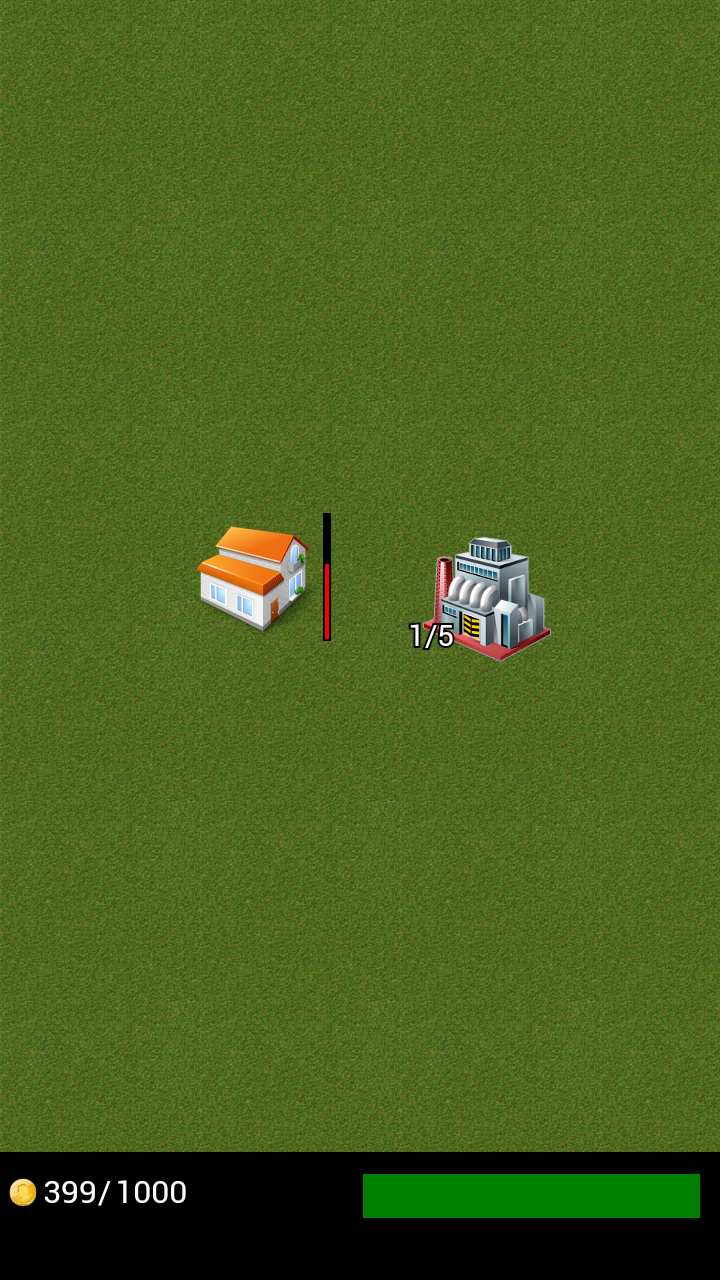
\includegraphics[scale=0.18]{pictures/sprint3-screen/buildPowerline_1.png}
		}
		\subfigure{
			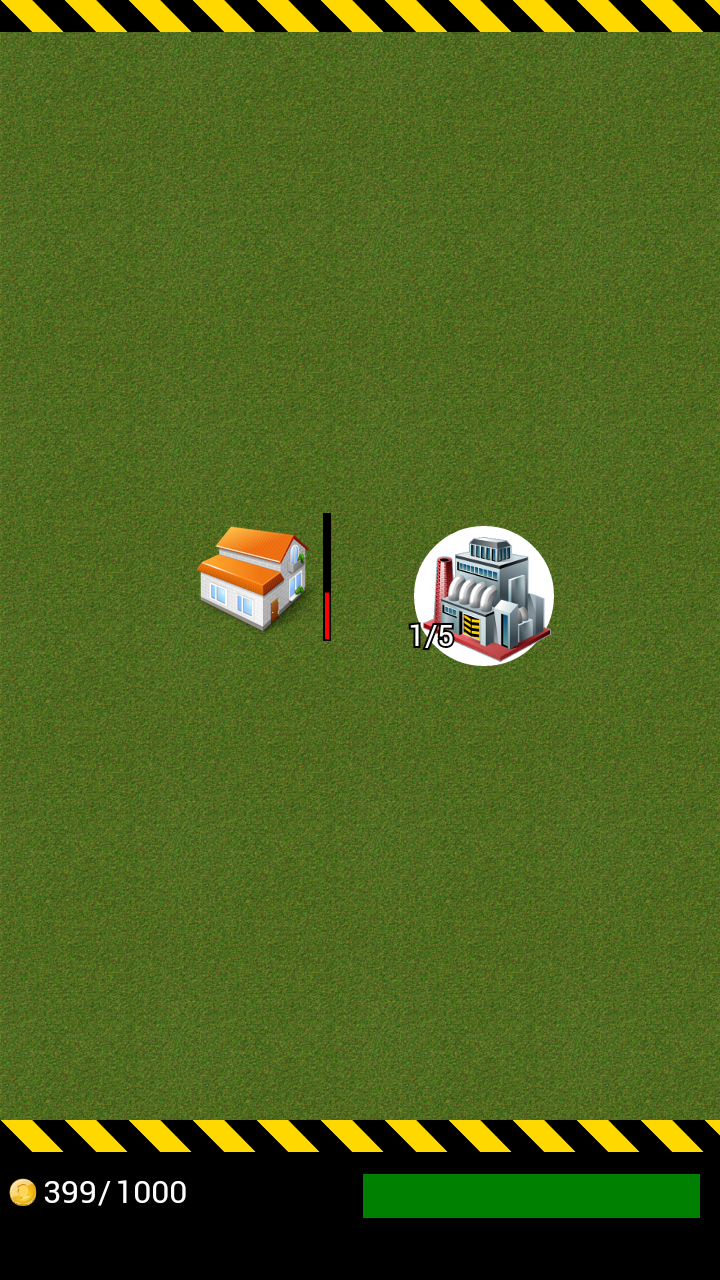
\includegraphics[scale=0.18]{pictures/sprint3-screen/buildPowerline_2.png}
		}
		\caption{User connecting buildings}
	\end{figure}
	\begin{figure}[H]
	\centering	
		\subfigure{
			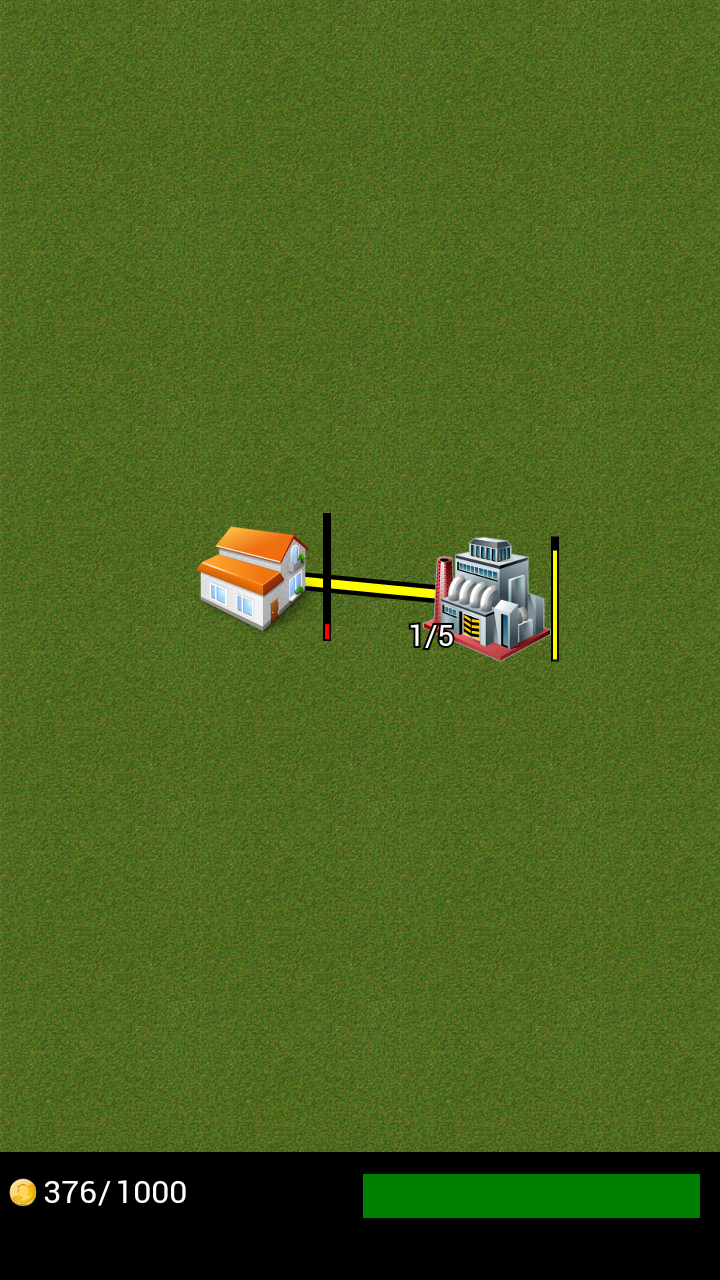
\includegraphics[scale=0.18]{pictures/sprint3-screen/buildPowerline_4.png}
		}
		\subfigure{
			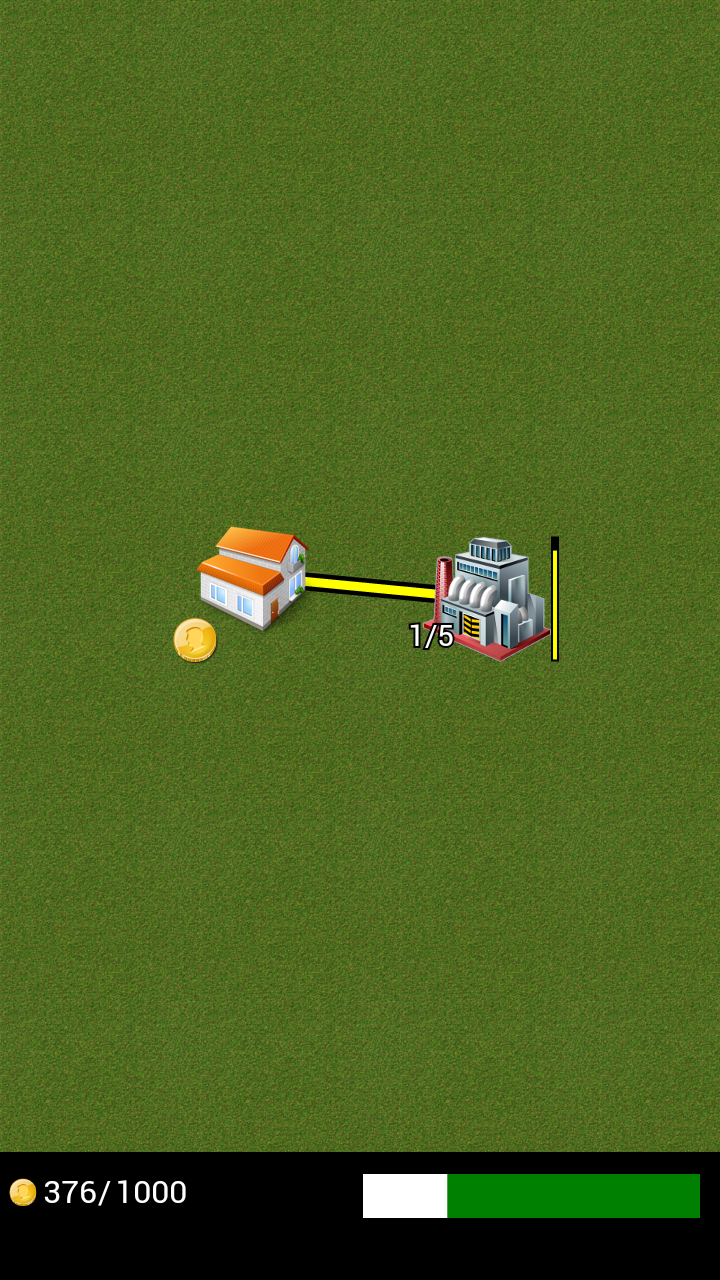
\includegraphics[scale=0.18]{pictures/sprint3-screen/buildPowerline_5.png}
		}
		\caption{Power is served and money can be collected}
	\end{figure}

	\begin{figure}[H]
		\centering
		\subfigure{
			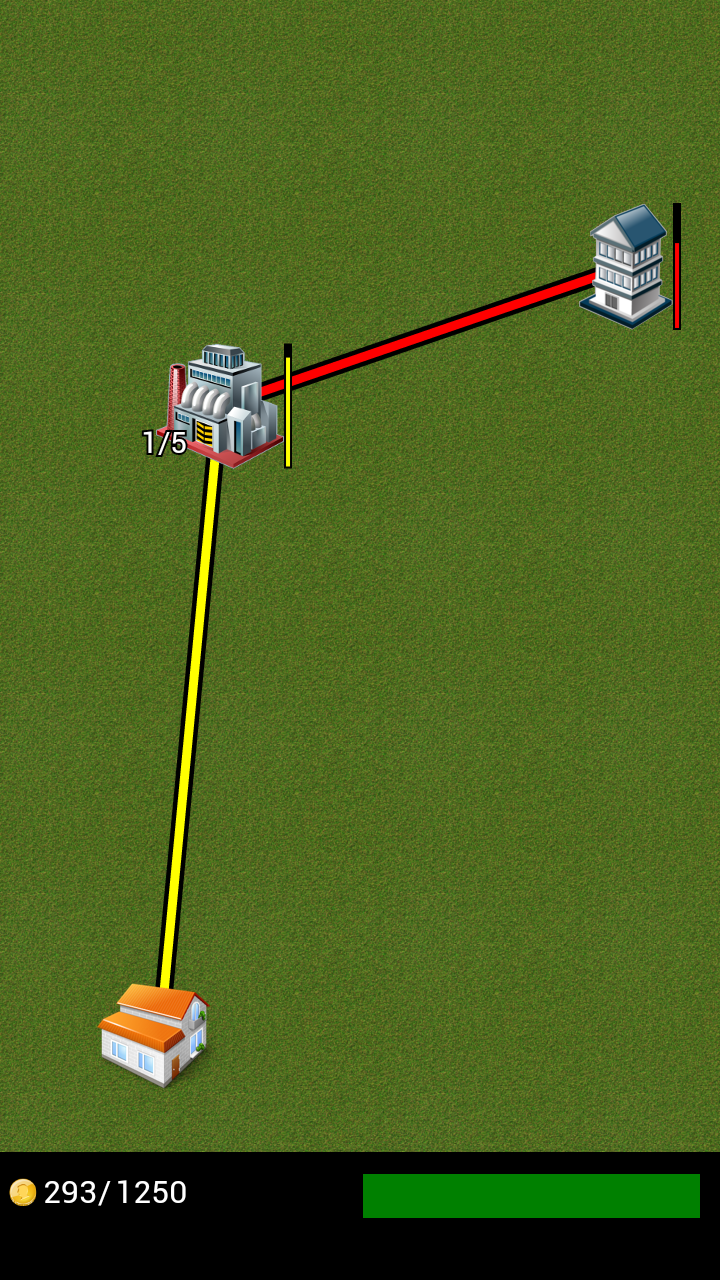
\includegraphics[scale=0.18]{pictures/sprint3-screen/damaged.png}
		}
		\subfigure{
			
\includegraphics[scale=0.18]{pictures/sprint3-screen/nextLevel.png}
		}
		\caption{Damaged red powerline and next level screen}
	\end{figure}

	\begin{figure}[H]
		\centering
		\subfigure{
			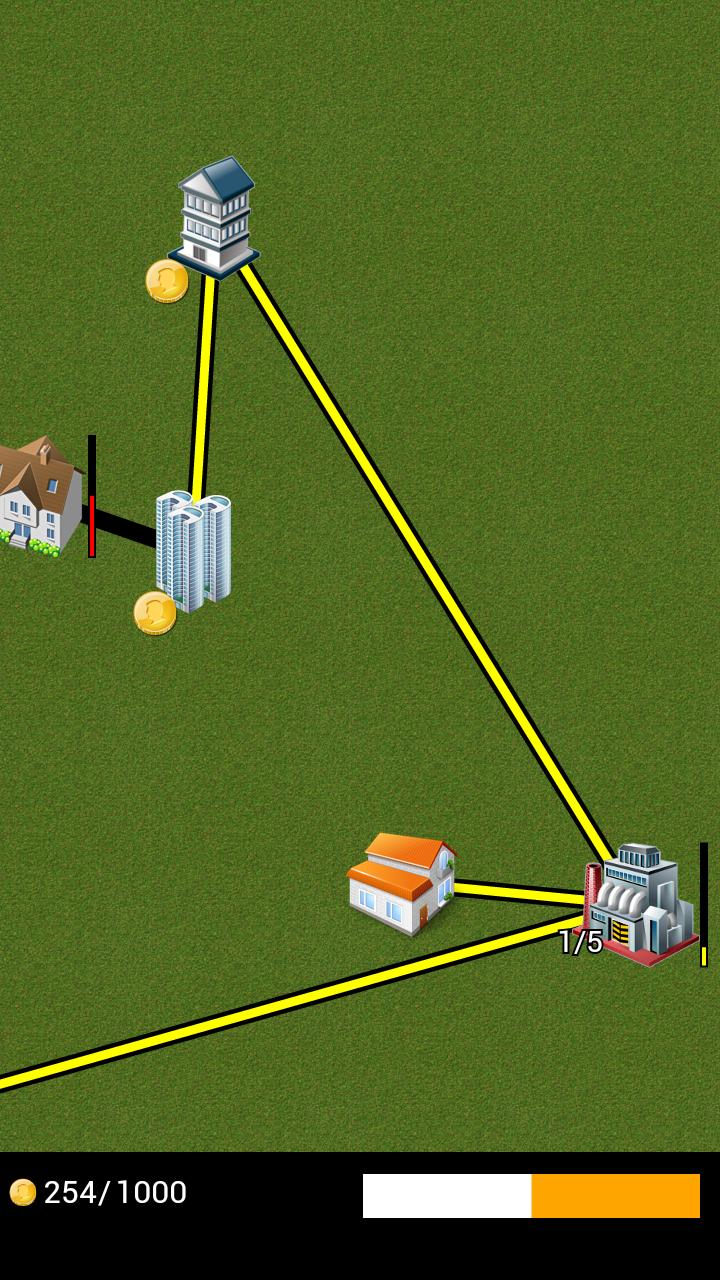
\includegraphics[scale=0.18]{pictures/sprint3-screen/notServe.png}
		}
		\subfigure{
			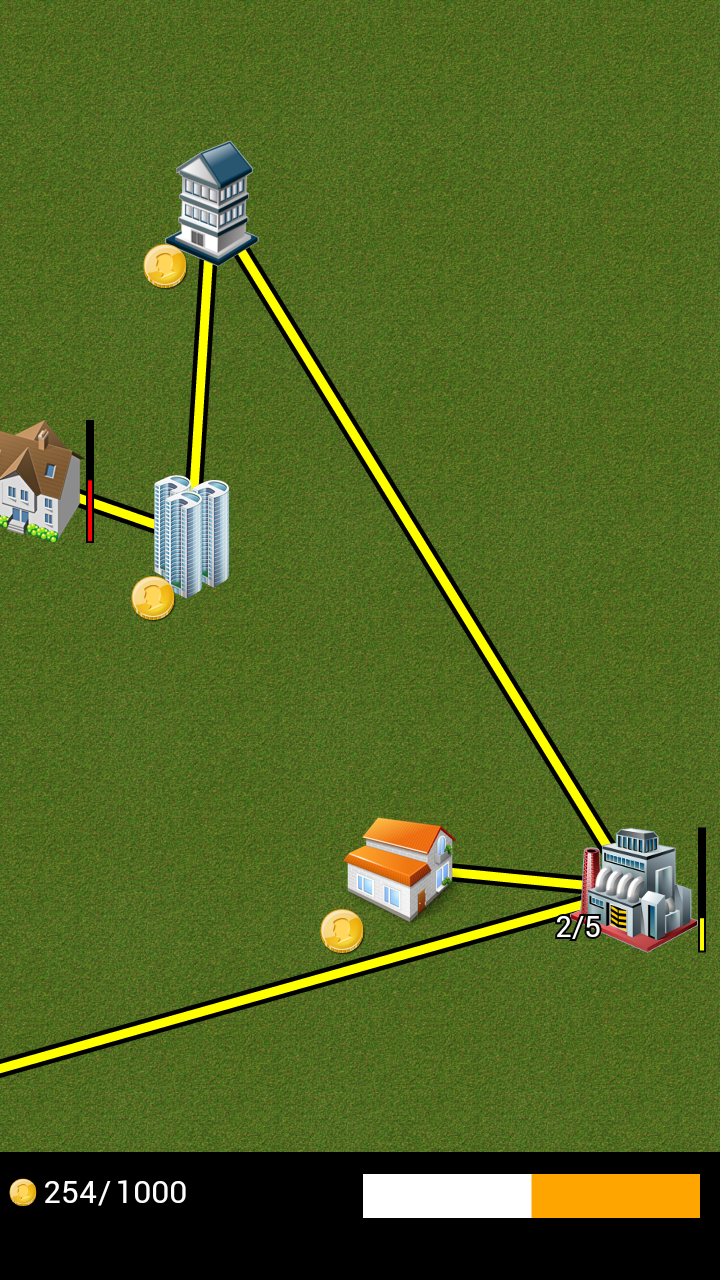
\includegraphics[scale=0.18]{pictures/sprint3-screen/serve.png}
		}
		\caption{Upgrade Powerplants to deliver more power}
	\end{figure}

	\subsection*{Algorithms}
		\begin{itemize}
			\item{\bf Breadth First Search}
			Breadth First Search is a standard algorithm taught in both Discrete Mathematics and 
			Algorithm courses. Breadth First Search (from now on refered to as BFS) traverses a graph 
			by exploring one level of the graph at a time. BFS is used to distribute power from the 
			power plants to the buildings on the map. The graph is defined by having all buildings 
			and power plants be vertices and the power lines are edges. The algorithm runs once for 
			each power plant on the map every time there is a change to the graph.

			\item {\bf Point to Line Segment Distance}
			The Point to Line Segment Distance algorithm works by projecting the point \emph{p} onto the line 
			defined as going through the point \emph{v} and the point \emph{w}. Then the algorithm 
			examines the following three different locations for the projection on the line: 
			\begin{enumerate}
				\item Before \emph{v}.
				\item After \emph{w}.
				\item Between \emph{v} and \emph{w}.
			\end{enumerate}
			If the projection lies before \emph{v} on the line, then the distance from \emph{p} to 
			the line segment from \emph{v} to \emph{w} is simply the distance from \emph{p} to 
			\emph{v}. If the projection lies after \emph{w} on the line, then the distance from 
			\emph{p} to the line segment is the distance from \emph{p} to \emph{w}. In the last case 
			where the projection lies between \emph{v} and \emph{w}, the answer is the distance from 
			\emph{p} to the location of the projection. There is also the special case where the 
			length of the line segment from \emph{v} to \emph{w} is 0. In that case the distance 
			from \emph{p} to the line segment is just the distance from \emph{p} to either \emph{v} 
			or \emph{w}.\cite{pldTheory}\cite{pldCode}

			\begin{figure}[H]
			\centering
			\subfigure{
				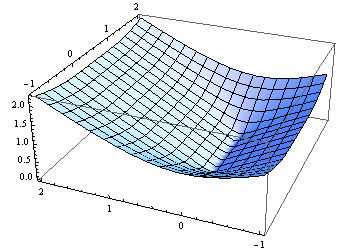
\includegraphics[scale=0.75]{pictures/PtLSplot}
			}
			\caption{Plot of Point to Line Segment Distance}
			\end{figure}
		\end{itemize}

\subsection{Functional Testing}

	The following test cases were executed at the end of this sprint:

	\definecolor{lightgray}{gray}{0.9}

	\begin{table}
	\begin{tabular}{| p{3cm} | p{6.5cm} | p{2.5cm} |}
		\hline
		\rowcolor{lightgray}
		{\bf Test Case} & {\bf Result} & {\bf Pass/Retest} \\ \hline

	  	FT-14 Complete Level & Works as expected. & Pass. \\ \hline
	  	
	  	FT-15 Limited Power & Works as expected. & Pass. \\ \hline
	  	
	  	FT-16 Remove Power Line & Works as expected. & Pass. \\ \hline
	  		  	
	  	FT-17 Different Buildings & Works as expected. & Pass. \\ \hline

	  	FT-18 Damaged Power Lines & Power lines are damaged throughout the game, but are not possible 
	  	to fix at the moment. & Retest. \\ \hline
	  	
	  	FT-19 Enter next level & Works as expected. & Pass. \\ \hline

	  	FT-20 Appearance of buildings in new levels & Works as expected. & Pass. \\ \hline

	  	FT-21 More unstable power lines in new levels & Works as expected. & Pass \\ \hline

	  	FT-22 Selected houses & Works as expected. & Pass. \\ \hline

	  	FT-23 Color of power lines & Works as expected. & Pass. \\ \hline
	  	FT-24 Map size in new levels & Works as expected. & Pass \\ \hline

	\end{tabular}
	\caption{Functional tests from sprint 3}
	\end{table}

	The following test cases did not pass previous tests and were retested this sprint:

	\begin{table}
	\begin{tabular}{| p{3cm} | p{6.5cm} | p{2.5cm} |}
		\hline
		\rowcolor{lightgray}
		{\bf Test Case} & {\bf Result} & {\bf Pass/Retest} \\ \hline

		FT-02 Appearance of buildings & Building can still appear on top of each other & Retest. \\ \hline

	  	FT-05 Build Power Plants & The power plants are still possible to place on top of other buildings & Retest. \\ \hline

	  	FT-06 Build Power Lines & The power lines now cost money. It is still possible to build power lines that cross each other and it is still possible to connect several power lines to one building. & Retest. \\ \hline

	  	FT-07 Upgrade Power Plant & The amount of power the power plant can supply is now increased by an upgrade. & Pass. \\ \hline
	\end{tabular}
	\caption{Redone tests in sprint 3}
	\end{table}

\subsection{Usability Test}

	This sections presents the results from the usability test that was carried out in this sprint. The usability test proved to be very helpful in terms of increasing the user friendliness of the user interfaces and making the game more enjoyable to play. More information on how the usability test was planned and carried out can be found in chapter 7.5 Usability Test.

	\subsubsection*{How far the game was from completion}

	The most apparent missing feature in the game at the time of testing was the possibility 
	to fix damaged power lines. At this point a damaged power line had to be removed and then 
	rebuilt. There are still no boundaries for where buildings can appear within the map, or 
	where power plants can be placed. Another aspect that affected the testing was that the balance 
	between the game parameters, for a given level, were not optimal as this was something that 
	would be difficult and time consuming to get just right. The parameters are the rate at which 
	buildings appear, the rate at which the health bar decreases when a building disappears, 
	how long it should take for a house without electricity to disappear, how much power a power 
	plant should be able to serve and how much effect an upgrade should have, and lastly how much 
	building should cost and how much money one should earn from the households. One game parameter 
	that affected the testing was the fact that the health bar decreased extremely slowly, a house 
	disappearing had almost no effect on the health bar. The objective was to not get a game over too fast, 
	and to not stress the testers while playing so that they had time to give us their thought 
	while playing. When looking back the health bar could have decreased faster and still not 
	make the game end too fast. Other features that were not implemented but did not noteworthy 
	affect the testing was high score, pausing the game and sounds.

	\subsubsection*{Feedback from the usability test}%\mbox{}\\

		\textbf{Zooming}
			Some testers found double tapping to zoom non-intuitive, and some wished it had 
			been possible to zoom by placing the thumb and pointer finger at opposing points 
			of the screen and moving the fingers away from each other.

			Several people wished it was possible to build also in zoomed-out mode.

		\textbf{The Hud}
			Those who had not read the game instructions in advance had trouble finding out that 
			the hud was possible to move up.

			Some people found the goal to be unclear and did not notice the "players money" vs. "goal" at the bottom of the screen.

			Several players did not understand what the health bar was, but when they were told what it was they understood it. A possible reason to why they did not understand that it was a health bar is explained in the section "How far the game was from completion".

		\textbf{The Coins}
			Several players ignored the coins because they did not know they had a function.

			All the players struggled with collecting money from the households. The reason for this was that they tapped the coin instead of the building and this lead to the money not being collected.

		\textbf{Power Lines}
			Many people had trouble understanding that the red power line indicated that the power line was damaged, and some thought it meant that there were not enough power.

			One person had trouble understanding that power line could be connected between buildings and connected them all directly to the power plant.

			At some points the players found it hard to tap the power line if it was to small.

		\textbf{Power Plants}
			It was not obvious to the players what the number on the power plant meant, i.e. the number indicating the number of upgrades done and the number of upgrades still available. Most of the players also did not understand that it was possible to upgrade the power plant, which might have led to the confusion about the numbers.

		\textbf{Buildings}
			Not everyone understood what the bar belonging to the house was, and some assumed that when the house disappeared they were punished in some way, but was unsure how. This may be caused by the fact that a disappearing house had little effect on the health bar.

			One player found it hard to play when buildings appeared very closed or almost on top of each other.

		\textbf{Other}
			At the very beginning of a new game, before the first house appeared nothing seemed 
			to be happening and this confused many of the testers.

			One player missed a sign telling him which level he was at.

			Some players wanted an in-game introduction to the different elements of the game and how it was played.

	\subsubsection*{Results of the Feedback}

	The following are suggestions to changes and improvements that should be made, as a result of the feedback from the usability test.

	Each level should start with an alert message that tells the player how much money he or she needs to earn in order to reach the next level. This will make the player more aware of what the goal is and that it is changing and will hopefully make the start of a new game less confusing.

	The zoomed out mode was intended for just giving an overview of the state of the game, making the game a little harder considering that the player did not know of all buildings needing power at all time, but if the possibility to build in zoomed-out mode will make the game more enjoyable, then this will be done.

	There should be an indication that the hud can be lifted into view, such as some form of handle, but considering the feedback from the customer, the building icons should always be visible in game mode to make building more effectively, thus solving both issues. One user liked that the hud was not visible because this made more room for the map, but we will strive to make the icons not clogging the screen.

	When collecting money, it is obviously more intuitive to tap the coin as opposed to the building. The coin will be moved closer to the building, so that when tapping the coin, the building will also be tapped, and as a result the money will be collected.

	It should be made clearer to the player that a power line is damaged. This can be done by making a cut to it. It should still be red to attract the attention of the player.

	In order to make it more visible to the player that the power plants can be upgraded, an arrow of some sort should be placed over the building.

	Which level the player is at should be visible when playing.

	\subsubsection*{Result of usability survey}

	The table below shows the average score for a given question or statements along with an explanation to the scale for the specific question. The question form as presented to the users can be found in Appendix F.

	\begin{table}[H]
	\begin{tabular}{| l | p{5cm} | p{1cm} | p{5cm} |}
  		\hline
		\rowcolor{gray}
		{\bf Nr.} & {\bf Question} & {\bf Avg Score} & {\bf Scale} \\ \hline
		
		1. & I think that I would like to play this game frequently. & 2.75 & 1 = not frequently, 5 = frequently\\ \hline

		2. & I found the game unnecessarily complex. & 2 & 1 = not complex, 5 = complex \\ \hline

		3. & I thought the game was easy to understand. & 3.5 & 1 = hard to understand, 5 = easy to understand \\ \hline

		4. & I thought there was too much inconsistency in this game. & 2 & 1 = not inconsistent, 5 = inconsistent \\ \hline

		5. & I would imagine that most people would learn to play this game very quickly. & 4 & 1 = not easy to learn, 5 = easy to learn \\ \hline

		6. & I found the game very cumbersome to play. & 2.5 & 1 = not cumbersome, 5 = cumbersome \\ \hline

		7. & I felt very confident playing the game. & 3.25 & 1 = not confident, 5 = confident \\ \hline

		8. & I needed to learn a lot of things before I could start playing the game. & 2.75 & 1 = needed to learn a lot, 5 = did not need to learn a lot \\ \hline

		9. & Game Instructions/Rules. & 2 & Simple - Average - Complex \\ \hline

		10. & Luck vs. Skill. & 4 & Pure luck - Average - All skill \\ \hline

		11. & How much did you like the graphics? & 4 & Did not like - OK - Loved \\ \hline

		12. & Game Idea (Concept). & 3.75 & Boring - OK - Terrific \\ \hline

		13. & How much did you like this game? & 3.5 & Hated it - OK - Loved it \\ \hline

		14. & How often would you play this game? & 2.5 & Never again - Now and then - A lot \\ \hline

		15. & Options for what you can do in the game. & 2.5 & Not enough - Just right - Too many \\ \hline

		16. & Game map size. & 3 & Too small - Just right - Too big \\ \hline

		17. & Game elements (size). & 3 & Too small - Just right - Too big \\ \hline

		18. & Text size. & 3 & Too small - Just right - Too big \\ \hline
	\end{tabular}
	\caption{Results of usability survey}
	\end{table}

	It needs to be stated that only 5 users answered this survey, and in order to smooth over the 
	variability in the individual differences in the users, we should have had at least 20 of them. 
	\cite{quantitativeTest} That does not mean that the numbers gathered holds no value and we will take a look at some of them. 

	All in all the scores are quite centered around the middle score of 3. If we look at how much or frequently the users thought they would play it the score was a little below the average "Now and then". If we look at how easy the game was to understand, they thought the game was above average easy to understand, and they thought people would learn how to play the game quite quickly. The users found the game a little below average cumbersome, and quite easy to play. They were quite positive to the game idea and their thought on how much the liked the game was a little above "OK".

	Many of the scores could have been better, this was however only an unfinished prototype of the game, still with bugs, and several improvements was made to the game after the feedback from the testers. These changes could hopefully make the game easier to understand and less cumbersome to play and subsequently more fun.

\subsection{Changes to the Requirements}

	The first change to the requirements during sprint 3 was the change of priority in requirement FR 1.2. The priority was changed from high to medium, because it is not an essential feature to have in order to have a working game, but can still be an improvement in the user experience.

	The requirements FR 6.5 and FR 3.5 were duplicates and were removed. The visual notification will not be implemented. The group defined a sound as a notification and added requirement FR 1.13.

	Other requirements were also added as the group discovered that they were either missing or would be an improvement to the design.
	
	\begin{table}[H]
	\begin{tabular}{| p{1.5cm} | p{12cm} |}
		\hline
		\rowcolor{lightgray}
		{\bf FR} & {\bf Change} \\ \hline
		FR 1.2 & {\bf \color{orange}[CHANGED PRIORITY FROM HIGH TO MEDIUM]} The user should be able 
		to exit the game at any time, and the game state should be saved and loaded when the user 
		returns to the game \\ \hline
		FR1.13 & {\bf \color{green}[NEW]} The user should get a sound notification of when new obstacles appear. \\ \hline
		FR3.5 & {\bf \color{red}[REMOVED]}  The user should get a notification of new obstacles outside the screen. \\ \hline
		FR 4.6 & {\bf \color{green}[NEW]} The user should be able to win the game by reaching the goal in the current level. The goal is level specific. \\ \hline
		FR 6.5 & {\bf \color{red}[REMOVED]} The user should get a notification of new events outside 
		the screen \\ \hline
		FR 6.11 & {\bf \color{green}[NEW]} The user should be able to see which houses is selected when building power cables. \\ \hline
		FR 6.12 & {\bf \color{green}[NEW]} The cables should change color if it is connected to a power 
		station. \\ \hline
		FR 6.13 & {\bf \color{green}[NEW]} The user should be able to see how much power the 
		power plant have left. This bar should decrease if a building is connected to the power plant 
		and should be increase if a building is removed. The colors should be yellow whit white 
		background. \\ \hline
	\end{tabular}
	\caption{Changes to version 3 of the requirement specification}
	\end{table}

\subsection{Group Dynamics}
	As a group, it is important to have fun. In the start of the project, the group had some
	problems with the communication, but this is not a problem anymore.
	When the group work we talk about what we read on reddit, what we did yesterday and 
	"bully" each other for funny writing typo, if found, in this report. 

	The harmony in the group is now great and it helps us keep up the good work and meet 
	our sprint goals. We believe having fun is the key to succeed in this project. 

\subsection{Customer Feedback}

	Before the sprint 3 delivery meeting the customer was provided with a presentation 
	of the game instructions as well as a newly updated playable game. The customer had 
	therefore been able to play the game in advance and had made up some thoughts about 
	the current state of the game. Their first concern was that it is tiresome and not 
	optimal to slide up the building menu every time one would want to build power plants 
	and power lines. A solution to this would be to keep the building icons on the screen 
	continuous. The second problem was that one would often like to build several power 
	lines in one go. With the current solution this is not optimal as the player has to 
	press the power line icon for each new power line. A solution to this could be to let 
	the player exit the building mode on own initiative and be able to build power lines as 
	long as he or she is in building mode.

\subsection{Sprint Retrospective}
	In this sprint, we did not do the sprint retrospective, but all the team members did
	get the chance to add changes to the next and last sprint. We are quite pleased with the way 
	we work and none of the group members had anything specific to add or remove in the next sprint.

	We have had one situation where two of the team members worked on the same implementation, 
	but we don't think that would happened again and have not been a problem up until now. 
	The group need to ensure a good communication within the group as well as give good status
	updates while working. 

	The group agreed to keep up the good work. "Team spirit!".
